\chapter{Fahrzeugdetektion}



\section{Programmablauf}

\begin{figure}
 \centering
 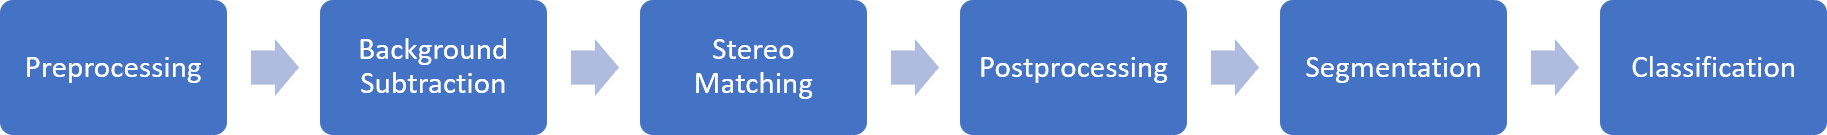
\includegraphics[width=1.1\textwidth]{media/pipeline.png}
 \caption{Pipeline zur Detektion}
 \label{fig:detection_programpipeline}
\end{figure}

\begin{figure}
 \centering
 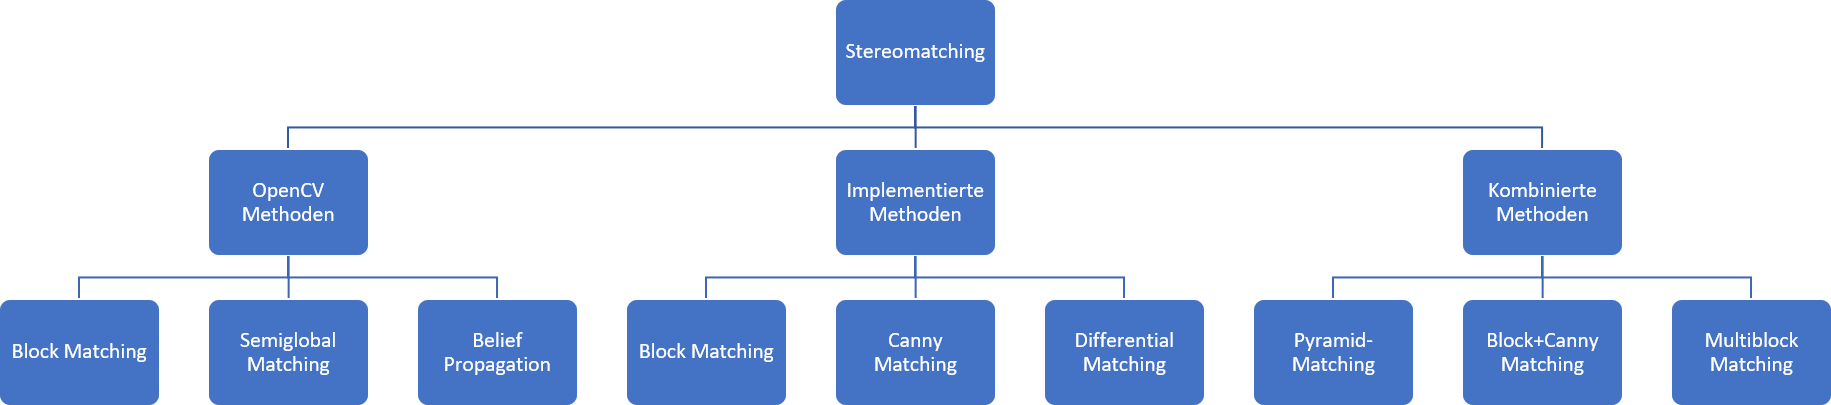
\includegraphics[width=1.1\textwidth]{media/detection/stereomatcher.png}
 \caption{Pipeline zur Detektion}
 \label{fig:detection_stereomatcher}
\end{figure}

\section{3D-Grafik}
\begin{figure}
 \centering
 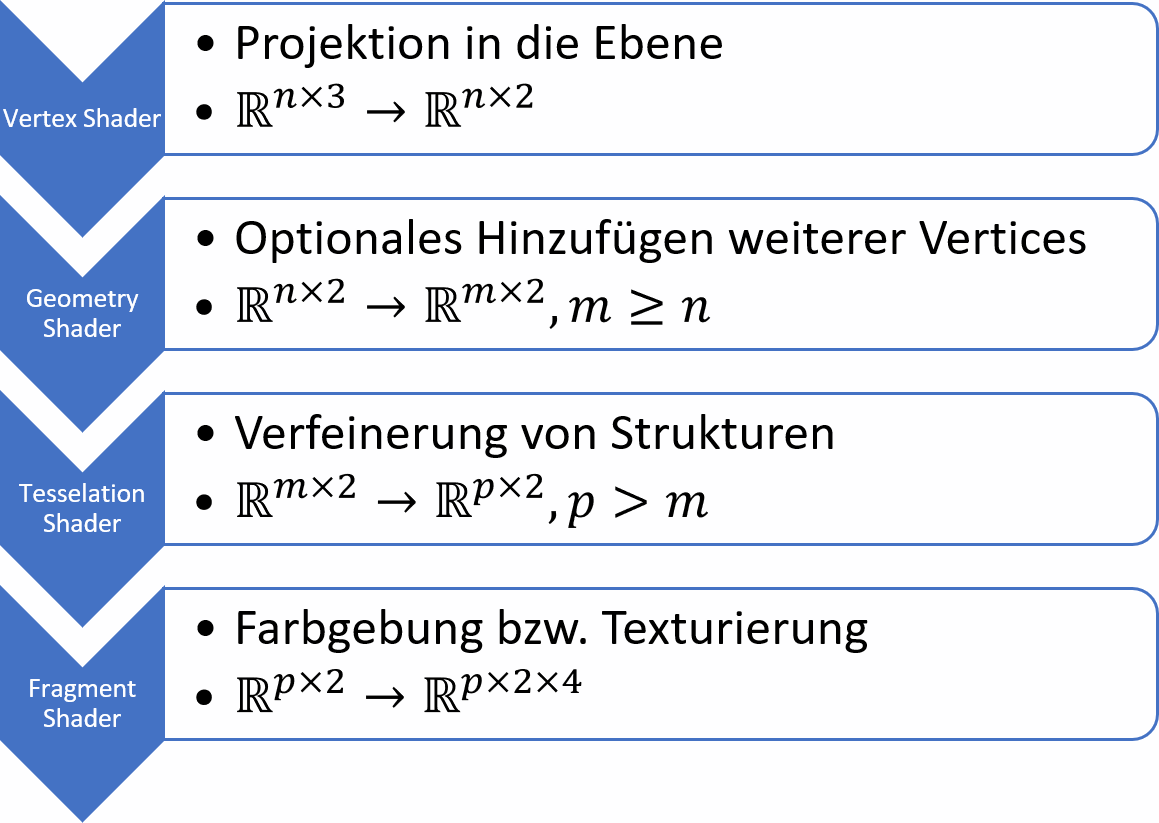
\includegraphics[width=1.1\textwidth]{media/detection/graphics_pipeline.png}
 \caption{Pipeline zur Detektion}
 \label{fig:detection_graphicspipeline}
\end{figure}

\section{Evaluation}

\subsection{Fehlernormen}

\(d_C(x, y) \) berechnete Disparity Map
\(d_T(x, y) \) Ground Truth Map

Bad Pixel Percentage

\begin{equation}
 P = \frac{1}{N} \sum_{(x, y)}(|d_C(x, y)-d_T(x, y)|>\delta_d)
\end{equation}

\(\delta_d \) Fehlertoleranz

Root Mean Squared Error
\begin{equation}
 E = \bigg( \frac{1}{N}\sum_{(x, y)}|d_C(x, y)-d_T(x, y)|^2 \bigg)^{\frac{1}{2}}
\end{equation}
